%
% svd.tex -- Singulärwertzerlegung
%
% (c) 2009 Prof Dr Andreas Mueller, Hochschule Rapperswil
%
\section{Singulärwertzerlegung\label{section-svd}}
\rhead{Singulärwertzerlegung}
\index{Singulärwertzerlegung}
\index{Zerlegung!Singulärwerte}
In der QR-Zerlegung unterscheidet sich von der LR-Zerlegung
dadurch, dass die Matrix $Q$ orthogonal ist, während $L$ eine
untere Dreiecksmatrix ist.
Kann man die LDU-Zerlegung so verallgemeinern,
dass $L$ und $R$ durch orthogonale Matrizen ersetzt
werden können?  Eine solche Zerlegung existiert tatsächlich,
und sie ist besonders nützlich, um das Eigenwertproblem
(Kapitel \ref{chapter-eigen}) zu lösen.


\subsection{Motivation
\label{subsection:svd:motivation}}
Abbildung~\ref{figure:svdmotivation} illustriert, wie man sich die 
Singulärwertzerlegung vorstellen kann.
Eine lineare Abbildung $\mathbb{R}^2\to\mathbb{R}^3$ mit Abbildungsmatrix
$A$ bildet den Einheitskreis  in $\mathbb{R}^2$ auf eine Ellipse in
$\mathbb{R}^3$ ab.
Um die Abbildung $A$ zu beschreiben, muss man zunächst die Halbachsen
der Ellipse kennen, also die Faktoren $s_1$ und $s_2$, um den gewisse
Radien des Einheitskreises gestreckt werden.
Dann braucht man die Richtungen der grössten und kleinsten Ausdehnung
der Ellipse, die mit $\vec{u}_1$ und $\vec{u}_2$ bezeichnet werden.
Sie stehen senkrecht aufeinander. 
Man kann sie mit einem Vektor $\vec{u}_3$ zu einer Orthonormalbasis
von $\mathbb{R}^3$ erweitern.
Schliesslich muss man wissen, welche Richtungen auf dem Einheitskreis
auf die Richtungen $\vec{u}_1$ und $\vec{u}_2$ abgebildet werden,
sie sind in Abbildung~\ref{figure:svdmotivation} mit $\vec{v}_1$ und
$\vec{v}_2$ bezeichnet.

Um die Abbildung aus diesen Informationen zu rekonstruieren, muss man
von einem gegeben Vektor $\vec{x}\in\mathbb{R}^2$ erst die Koordinaten im
Koordinatensystem zur Basis $\mathcal{V}=\{\vec{v}_1,\vec{v}_2\}$ ermitteln.
Dies geschieht, indem man die Skalarprodukte $\vec{v}_1\cdot \vec{x}$ und
$\vec{v}_2\cdot \vec{x}$ ausrechnet.
In Matrixnotation sind dies
$\vec{v}_1^t\vec{x}$
und
$\vec{v}_2^t\vec{x}$,
was man in einer Matrixoperation $V^t\vec{x}$ zusammenfassen kann, wenn
man die Vektoren $\vec{v}_1$ und $\vec{v}_2$ als Spalten in die 
$2\times 2$-Matrix $V$ schreibt.
Da die Vektoren $\vec{v}_i$ eine Orthonormalbasis bilden, ist $V$ eine
orthogonale Matrix.

\begin{figure}
\centering
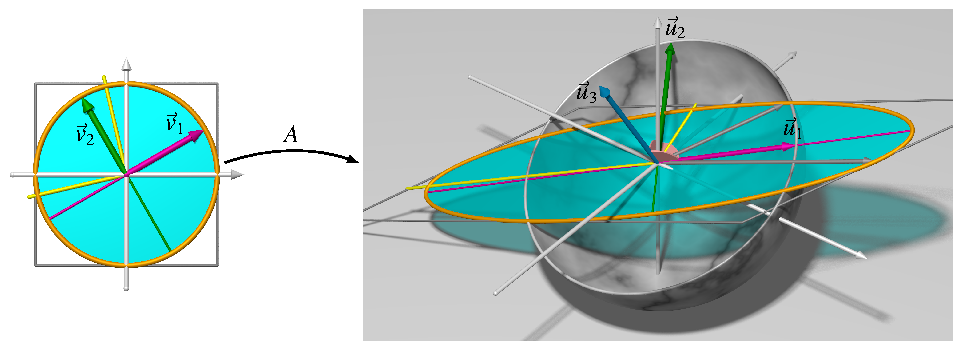
\includegraphics[width=\textwidth]{7/images/svdmotivation.pdf}
\caption{
Konstruktion der Singulärwertzerlegung einer linearen Abbildung mit
der Matrix $A$.
$A$ bildet den Einheitskreis in $\mathbb{R}^2$ auf eine Ellipse
in $\mathbb{R}^3$ ab.
Die Länge der Halbachsen der Ellipse sind die Singulärwerte $s_1$ und $s_2$ 
von $A$.
Die Richtungen $\vec{u}_1$ und $\vec{u}_2$  der Halbachsen 
können durch $\vec{u}_3$ zu einer orthonormierten Basis von
$\mathbb{R}^3$ ergänzt werden.
Die Vektoren $\vec{v}_1$ und $\vec{v}_2$ werden von $A$ auf die
Halbachsenrichtungen $\vec{u}_1$ und $\vec{u}_2$ abgebildet.
Die Singulärwertzerlegung erhält man dann, indem man die Vektoren 
$\vec{v}_i$ als Spalten in eine Matrix $V$ und die Vektoren $\vec{u}_j$
als Spalten in eine Matrix $U$ schreibt.
Zusammen mit der Matrix $S$ aus \eqref{eqn:svd:Smatrix} erhält man
die Zerlegung $A=USV^t$.
\label{figure:svdmotivation}
}
\end{figure}

Das Produkt $V^t\vec{x}$ liefert die Koordinaten von $\vec{x}$
bezüglich der Basis $\mathcal{V}$.
Diese Koordinaten werden jetzt um die Faktoren $s_1$ und $s_2$ 
gestreckt und sollen die Koordinaten eines Punktes in $\mathbb{R}^3$
bezüglich der Basis $\mathcal{U}=\{\vec{u}_1,\vec{u}_2,\vec{u}_3\}$ ergeben.
Die $\vec{u}_3$-Komponente ist immer $0$, daher ist die zu diesem
Schritt gehörige Abbildungsmatrix
\begin{equation}
S=\begin{pmatrix}
s_1& 0 \\
 0 &s_2\\
 0 & 0
\end{pmatrix}.
\label{eqn:svd:Smatrix}
\end{equation}

Die Koordinaten $SV^t\vec{x}$ bezüglich der Basis $\mathcal{U}$
müssen jetzt in einen Vektor in $\mathbb{R}^3$ umgerechnet werden.
Schreibt man die Vektoren $\vec{u}_i$ in die Spalten der Matrix $U$,
dann wird dies durch das Produkt $USV^t\vec{x}$ erreicht.
Da $\mathcal{U}$ eine Orthonormalbasis ist, ist $U$ eine orthogonale
Matrix.


\begin{satz}[Singulärwertzerlegung]\label{satz-svd}
Sei $A$ eine $m\times n$-Matrix mit Rang $r$.
Dann gibt es eine orthogonale $m\times m$-Matrix $U$, eine
orthogonale $n\times n$-Matrix $V$ und eine $m\times n$-Diagonalmatrix
mit Rang $r$ 
\begin{equation}
S=\left(
\begin{tabular}{>{$}c<{$}>{$}c<{$}>{$}c<{$}|>{$}c<{$}>{$}c<{$}>{$}c<{$}}
s_1   &\dots &0     &0     &\dots &0\\
\vdots&\ddots&\vdots&\vdots&\ddots&\vdots\\
0     &\dots &s_r   &0     &\dots &0\\
\hline
0     &\dots &0     &0     &\dots &0\\
\vdots&\ddots&\vdots&\vdots&\ddots&\vdots\\
0     &\dots &0     &0     &\dots &0\\
\end{tabular}
\right)
\label{s-matrix}
\end{equation}
mit $s_1\ge s_2\ge\dots \ge s_r$ und $A=USV^t$.
\end{satz}

\subsection{Berechnung der Singulärwertzerlegung
\label{subsection:berechnungdersingulaerwertzerleung}}
Im folgenden nehmen wir an, dass die Matrix $A$ eine Singulärwertzerlegung
$A=USV^t$ hat.
Das Produkt $A^tA$ ist
\[
A^tA
=
(USV^t)^tUSV^t
=
VS^t\underbrace{U^tU}_{=E}SV^t
=
VS^tSV^t
=
V
\begin{pmatrix}
s_1^2 &  0   & \dots &  0   &  0   &\dots\\
  0   &s_2^2 & \dots &  0   &  0   &\dots\\
\vdots&\vdots&\ddots &\vdots&\vdots&     \\
  0   &  0   & \dots & s_r^2&  0   &\dots\\
  0   &  0   & \dots &   0  &  0   &\dots\\
\vdots&\vdots&       &\vdots&\vdots&\ddots
\end{pmatrix}
V^t
\]
Die orthogonale Matrix $V^t$ transformiert also die symmetrische Matrix
$A^tA$ auf Diagonalform.
In der Eigenwertheorie (Kapitel~\ref{chapter-eigen}) wird gezeigt,
dass es zu jeder symmetrischen Matrix eine orthogonale Matrix
gibt, die sie auf Diagonalform transformiert
(Satz~\ref{satz:symmetrischdiagonalisierbar}).
In den Spalten der Matrix $V$ stehen dann Eigenvektoren von $A^tA$,
die Eigenwerte sind die $s_i^2$ oder $0$.

Für die Matrix $U$ gilt natürlich dasselbe.
Das Produkt
\[
AA^t
=
USV^tVS^tU^t
=
USS^tU^t
\]
zeigt, dass $U^t$ die symmetrische Matrix $AA^t$ auf Diagonalform
transformiert.

Die Matrizen $U$ und $V$ sind allerdings nicht eindeutig.
Dies kann man schon am Motivationsbeispiel in
Abbildung~\ref{figure:svdmotivation} erkennen.
Die Vektoren $\vec{u}_1$ und $\vec{u}_2$ waren als die Richtungen
der grössten und kleinsten Ausdehnung der Ellipse festgelegt,
aber $-\vec{u}_1$ und $-\vec{u}_2$ erfüllen diese Bedingung auch.
Wenn zwei Singulärwerte gleich sind, zum Beispiel weil sie 0 sind,
dann kann man eine beliebige Drehung in der von den Vektoren aufgespannten
Ebene durchführen und erhält ebenfalls anwendbare Vektoren.
Man muss daher separat sicherstellen, dass die $\vec{u}_i$ tatsächlich
die Bilder der Vektoren $\vec{v}_i$ unter der Abbildung $A$ sind.
Am einfachsten geht dies, wenn man den folgenden Algorithmus verwendet:
\begin{enumerate}
\item
Bestimme Vektoren $\vec{v}_i$ als Eigenvektoren von $A^tA$ mit
Eigenwerten $\lambda_i$.
Die Vektoren sollen so geordnet sein, dass 
\[
\lambda_1 \ge \lambda_2 \ge \dots \ge \lambda_r > 0
\]
gilt.
\item
Die Singulärwerte sind $s_i = \sqrt{\lambda_i}$
\item
Wähle $\vec{u}_i=A\vec{v}_i/|A\vec{v}_i|$ für $1\le i\le r$
\item
Wähle eine beliebige orthonormierte Basis von $\operatorname{ker} AA^t$
für die Vektoren $\vec{u}_{r+1},\dots,\vec{u}_m$.
\end{enumerate}
Für die Bestimmung der Eigenwerte und Vektoren wird auf
Kapitel~\ref{chapter-eigen} verweisen.

Die Berechnung der Singulärwertzerlegung kann in Octave/Matlab
mit der Funktion {\tt svd} erfolgen.
Sie liefert einen Vektor mit den Singulärwerten $s_1,\dots,s_n$ zurück.
Will man auch die Matrizen $U$ und $V$ bekommen, muss man als Rückgabewert
eine Matrix von Rückgabewerten spezifizieren
\begin{verbatim}
[U, S, V] = svd(A)
\end{verbatim}

\begin{beispiel}
Die Singulärwertzerlegung der Matrix $A$ aus dem letzten Beispiel 
bekommt man mit Octave:
\begin{verbatim}
> [U,S,V] = svd([9,3,3;3,17,21;3,21,107])
U =

   0.034813  -0.443841   0.895429
   0.217231  -0.871189  -0.440272
   0.975499   0.209842   0.066088

S =

Diagonal Matrix

   111.7835          0          0
          0    13.4702          0
          0          0     7.7464

V =

   0.034813  -0.443841   0.895429
   0.217231  -0.871189  -0.440272
   0.975499   0.209842   0.066088
\end{verbatim}
\end{beispiel}
\subsection{Pseudoinverse}
\index{Pseudoinverse}
Als Anwendung der Singulärwertzerlegung betrachten wir das Problem, eine Matrix
$A^\dagger$
zu finden, die ``so inverse wie möglich'' ist zu einer gegebenen
$n\times m$-Matrix $A$.
Natürlich können wir nicht erwarten, dass das Produkt $AA^\dagger$ 
oder $A^\dagger A$
eine Einheitsmatrix ergibt.
Wenn die Matrix $A$ den Rang $r$ hat, dann sollte auch $A^\dagger$ den Rang $r$
haben.
Ist der Rang nicht voll, dann könnten wir erwarten, dass das Produkt die Form
\[
P=
\begin{pmatrix}
1&      & & &      & \\
 &\ddots& & &      & \\
 &      &1& &      & \\
 &      & &0&      & \\
 &      & & &\ddots& \\
 &      & & &      &0\\
\end{pmatrix}
\]
mit genau $r$ Einsen in der linken oberen Ecke hat.
Man nennt $P$ eine {\em Projektionsmatrix}, sie hat die Eigenschaft $P^2=P$.
\index{Projektion}
\index{Projektionsmatrix}
Dies ist aber zu viel verlangt, ändert man nämlich das Koordinatensystem,
dann geht die spezielle Form der Matrix $P$ verloren.
Die Projektionseigenschaft $P^2=P$ ist jedoch unabhängig vom Koordinatensystem.
Ist nämlich $T$ eine Transformationsmatrix und $P'=TPT^{-1}$, dann gilt
\[
P'^2=TPT^{-1}TPT^{-1}=TPPT^{-1}=TPT^{-1}=P'.
\]

\begin{beispiel}
Die Matrix
\[
P=\begin{pmatrix}1&0\\0&0\end{pmatrix}
\]
ist eine Projektionsmatrix.
Dreht man das Koordinatensystem um den Winkel $\alpha$, wird die Matrix 
gemäss $P'=D_\alpha AD_\alpha ^{-1}=D_\alpha AD_\alpha^t$ transformiert:
\begin{align*}
P'&=
\begin{pmatrix}\cos\alpha&-\sin\alpha\\\sin\alpha&\cos\alpha\end{pmatrix}
\begin{pmatrix}1&0\\0&0\end{pmatrix}
\begin{pmatrix}\cos\alpha&\sin\alpha\\-\sin\alpha&\cos\alpha\end{pmatrix}
\\
&=
\begin{pmatrix}\cos\alpha&-\sin\alpha\\\sin\alpha&\cos\alpha\end{pmatrix}
\begin{pmatrix}\cos\alpha&\sin\alpha\\0&0\end{pmatrix}
\\
&=
\begin{pmatrix}\cos^2\alpha&\cos\alpha\sin\alpha\\\sin\alpha\cos\alpha&\sin^2\alpha\end{pmatrix}.
\end{align*}
Wir kontrollieren die Projektionseigenschaft:
\begin{align*}
P^{\prime 2}
&=
\begin{pmatrix}
\cos^2\alpha
	&\sin\alpha\cos\alpha\\
\sin\alpha\cos\alpha
	&\sin^2\alpha
\end{pmatrix}^2
\\
&=
\begin{pmatrix}
\cos^4\alpha + \sin^2\alpha\cos^2\alpha
	&\sin\alpha\cos^3\alpha+\sin^3\alpha\cos\alpha\\
\sin\alpha\cos^3\alpha+\sin^3\alpha\cos\alpha
	&\sin^2\alpha\cos^2\alpha+\sin^4\alpha
\end{pmatrix}
\\
&=
\begin{pmatrix}
(\cos^2\alpha + \sin^2\alpha)\cos^2\alpha
	&\sin\alpha\cos\alpha(\cos^2\alpha+\sin^2\alpha)\\
\sin\alpha\cos\alpha(\cos^2\alpha+\sin^2\alpha)
	&\sin^2\alpha(\cos^2\alpha+\sin^2\alpha)
\end{pmatrix}
\\
&=
\begin{pmatrix}
\cos^2\alpha
	&\sin\alpha\cos\alpha\\
\sin\alpha\cos\alpha
	&\sin^2\alpha
\end{pmatrix}=P'.
\end{align*}
\end{beispiel}

Wir können also nur erwarten, dass $A^\dagger A$ bzw.~$AA^\dagger$ die
Projektionseigenschaft haben.
Nur im Falle vollen Ranges wird eines der Produkte eine Einheitsmatrix sein.

In einfachen Fällen können wir eine Pseudoinverse sofort angeben.
Die Matrix $A$
\[
A=\begin{pmatrix}
2&0&0\\
0&3&0\\
0&0&0
\end{pmatrix}
\]
ist nicht invertierbar, weil sie nicht vollen Rang hat.
Aber die Matrix
\[
A^\dagger=\begin{pmatrix}
\frac12&0&0\\
0&\frac13&0\\
0&0&0
\end{pmatrix}
\]
ist in dem Sinne eine Inverse, dass $AA^{\dagger}$ und $A^\dagger A$ zwar keine
Einheitsmatrizen sind, aber doch mindestens Projektionsmatrizen mit dem gleichen
Rang wie $A$:
\begin{align*}
AA^\dagger=A^\dagger A
=
\begin{pmatrix}
1&0&0\\
0&1&0\\
0&0&0
\end{pmatrix}.
\end{align*}
Diesen Spezialfall wollen wir im Folgenden verallgemeinern.

Eine $m\times n$-Diagonalmatrix $S$ wie in (\ref{s-matrix}) in Satz~\ref{satz-svd}
hat als Pseudoinverse die $n\times m$-Matrix
\begin{equation}
S^\dagger=\left(
\begin{tabular}{>{$\displaystyle}c<{$}>{$\displaystyle}c<{$}>{$\displaystyle}c<{$}>{$\displaystyle}c<{$}|>{$}c<{$}>{$}c<{$}>{$}c<{$}}
\frac1{s_1}&           &      &           &     &      & \\
           &\frac1{s_2}&      &           &     &      & \\
           &           &\ddots&           &     &      & \\
           &           &      &\frac1{s_r}&     &      & \\
\hline
           &           &      &           &\quad&      & \\
           &           &      &           &     &     0& \\
           &           &      &           &     &      &\qquad
\end{tabular}
\right)
\end{equation}
denn die Produkte $S^\dagger S$ und $SS^\dagger$ sind beide Projektionsmatrizen
mit Rang $r$.
$S^\dagger S$ ist eine $n\times n$-Matrix, $SS^\dagger$ ist eine
$m\times m$-Matrix.

Mit Hilfe der Singulärwertzerlegung lässt sich diese Konstruktion
auf beliebige Matrizen verallgemeinern.
Sei $A$ eine $m\times n$-Matrix mit Singulärwertzerlegung
$A=USV^t$, wobei $U$ eine orthogonale $m\times m$-Matrix, $V$ eine orthogonale
$n\times n$-Matrix und $S$ eine $m\times n$-Diagonalmatrix wie in (\ref{s-matrix})
von Satz~\ref{satz-svd} ist.
Wir setzen
\begin{equation}
A^\dagger = VS^\dagger U^t,
\label{definition-pseudoinverse}
\end{equation}
$A^\dagger$ heisst die {\em Pseudoinverse} von $A$.

Wir überzeugen uns zunächst, dass $A^\dagger$ für invertierbare Matrizen
mit der gewöhnlichen Inversen $A^{-1}$ übereinstimmt.
Für invertierbares $A$ ist $n=m$ und $S$ ist eine Diagonalmatrix ohne Nullen
auf der Diagonalen.
Insbesondere gilt $S^\dagger=S^{-1}$, oder $S^\dagger S=SS^\dagger=E$.
Daher gilt auch
\begin{align*}
A^\dagger A&=VS^\dagger U^tUSV^t=VS^\dagger SV^t=VV^t=E\\
AA^\dagger &=USV^tVS^\dagger U^t=USS^\dagger U^t=UU^t=E,
\end{align*}
also ist $A^\dagger=A^{-1}$ in diesem Fall.

Im allgemeinen Fall gilt
\begin{align*}
A^\dagger A&=VS^\dagger U^tUSV^t=VS^\dagger SV^t=VP_1V^{-1}\\
AA^\dagger &=USV^tVS^\dagger U^t=USS^\dagger U^t=UP_2U^{-1},
\end{align*}
wobei die $P_i$ geeignete Projektionsmatrizen sind.
In einem geeigneten Koordinatensystem, das im Wesentlichen durch die Matrizen
$U$ bzw.~$V$ gegeben ist, sind die Produkte $A^\dagger A$ und $AA^\dagger$
also Projektionsmatrizen.
Anders ausgedrückt, soweit es möglich ist, also in den durch die Projektion
gegebenen Unterräumen, ist $A^\dagger$ eine Inverse von $A$.
$A^\dagger$ heisst die {\em Pseudoinverse} von $A$.

\begin{beispiel}
Die Matrix
\[
A=\begin{pmatrix}
1&2&9&1\\
2&0&1&5
\end{pmatrix}
\]
hat Rang $2$.
Wir berechnen die Pseudoinverse mit Hilfe von Octave, dazu bestimmen wir
zunächst die Singulärwertzerlegung:
\begin{verbatim}
> A = [1,2,9,1;2,0,1,5]
A =

   1   2   9   1
   2   0   1   5

> [U,S,V] = svd(A)
U =

  -0.96747  -0.25300
  -0.25300   0.96747

S =

Diagonal Matrix

   9.5490        0        0        0
        0   5.0809        0        0

V =

  -0.154305   0.331029  -0.751912  -0.548852
  -0.202631  -0.099587  -0.575830   0.785775
  -0.938335  -0.257732   0.182137  -0.141163
  -0.233789   0.902262   0.264337   0.247774
\end{verbatim}
Aus $S$ können wir jetzt die Pseudoinverse $S^\dagger$ berechnen:
\begin{verbatim}
> Sdagger = S';
> Sdagger(1,1)=1/S(1,1);
> Sdagger(2,2)=1/S(2,2)
Sdagger =

Diagonal Matrix

   0.10472         0
         0   0.19681
         0         0
         0         0
\end{verbatim}
Wir kontrollieren, ob sie die verlangte Projektionseigenschaft hat:
\begin{verbatim}
> Sdagger * S
ans =

Diagonal Matrix

   1   0   0   0
   0   1   0   0
   0   0   0   0
   0   0   0   0

> S * Sdagger
ans =

Diagonal Matrix

   1   0
   0   1
\end{verbatim}
Jetzt können wir mit Hilfe der Matrizen $U$ und $V$ auch die Pseudoinverse
$A^\dagger$ bestimmen.
\begin{verbatim}

> Adagger = V * Sdagger * U'
Adagger =

  -8.4962e-04   6.7120e-02
   2.5489e-02  -1.3594e-02
   1.0790e-01  -2.4214e-02
  -2.1240e-02   1.7799e-01

\end{verbatim}
Das Produkt $AA^\dagger$ muss eine Projektionsmatrix vom Rang $2$ sein, wir
berechnen
\begin{verbatim}
> A * Adagger
ans =

   1.0000e+00  -5.5511e-17
  -2.7756e-17   1.0000e+00
\end{verbatim}
im Rahmen der Rechengenauigkeit ist das tatsächlich eine Einheitsmatrix.

Das Produkt $A^\dagger A$ muss eine Projektionsmatrix sein, es muss also
für $P=A^\dagger A$ gelten, dass $P^2=P$ ist.
Wir berechnen mit Octave die Differenz $P^2-P$ und erhalten
\begin{verbatim}
> P = Adagger * A
P =

   0.1333900  -0.0016992   0.0594732   0.3347494
  -0.0016992   0.0509771   0.2158029  -0.0424809
   0.0594732   0.2158029   0.9468989  -0.0131691
   0.3347494  -0.0424809  -0.0131691   0.8687341

> P * P - P
ans =

   5.5511e-17  -1.7347e-18   1.3878e-17   1.1102e-16
  -1.2143e-17   6.9389e-18   0.0000e+00  -2.7756e-17
  -2.0817e-17   0.0000e+00   1.1102e-16  -7.2858e-17
   1.1102e-16  -1.3878e-17   0.0000e+00   3.3307e-16
\end{verbatim}
Im Rahmen der Rechengenauigkeit ist das $0$.
\end{beispiel}
